\section{Laboratory work implementation}

\subsection{Tasks and Points}

\par De creat o aplicație mobilă simplă ce va avea funcționalul unui cronometru.

\par Aplicația va avea următarele componente:
\begin{itemize}
 \item Un label în care se va arăta timpul;
 \item Un buton pentru a porni/opri cronometrul;
 \item Un buton pentru a înregistra valoarea curentă;
 \item Un buton pentru a reseta cronometrul;
 \item O listă în care vor fi păstrate rezultatele.
\end{itemize}

\subsection{Analiza lucrarii de laborator}

\par Link spre repozitoriu: \url{https://your.link.goes.here}

\par Platforma Android\cite{android} a dictat mediul de dezvoltare și limbajul de programare utilizate, deci au fost utilizate Android Studio\cite{studio} și Java. 

\par Aplicația constă dintr-un \textit{Activity} pe care sunt amplasate toate elementele de UI necesare: un label, trei butoane și lista de păstrare a rezultatelor intermediare.

\par Când utilizatorul atinge butonul \textit{Start}, se pornește un timer care actualizează textul din label cu o anumită periodicitate. În timp ce cronometrul lucrează, este activ butonul \textit{Lap}. La atingerea lui, valoarea curentă a cronometrului este înscrisă în listă. Când este atins butonul \textit{Reset}, toate datele se șterg și cronometrul se resetează la zero. 


\subsection{Imagini}

\begin{figure}[ht]
	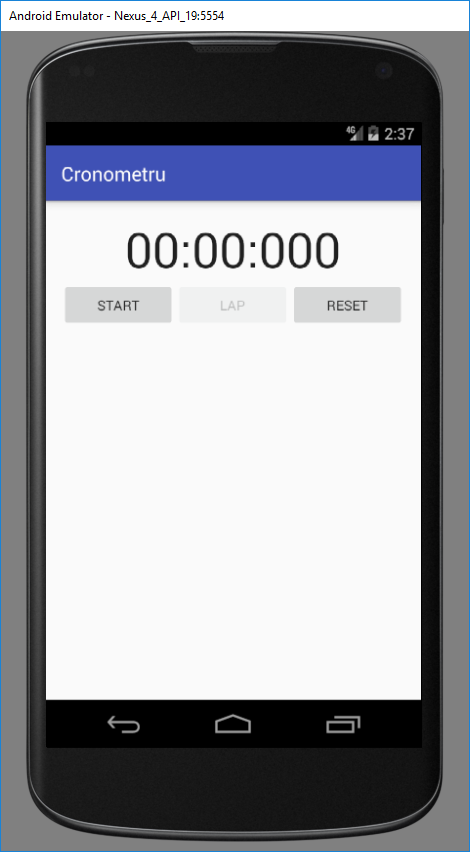
\includegraphics[scale=0.35]{imagini/1-initial}
	\centering
	\captionof{figure}{Ecranul inițial}
\end{figure}

\begin{figure}[ht]
	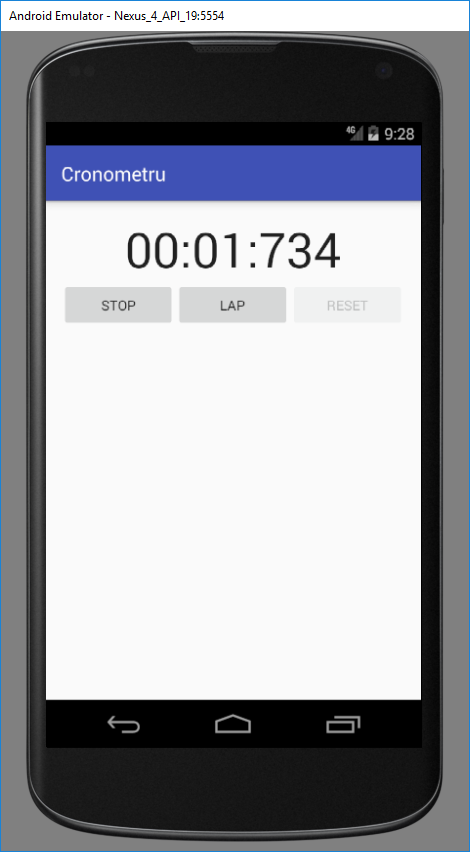
\includegraphics[scale=0.5]{imagini/2-start}
	\centering
	\captionof{figure}{Cronometrul pornit}
\end{figure}

\begin{figure}[ht]
	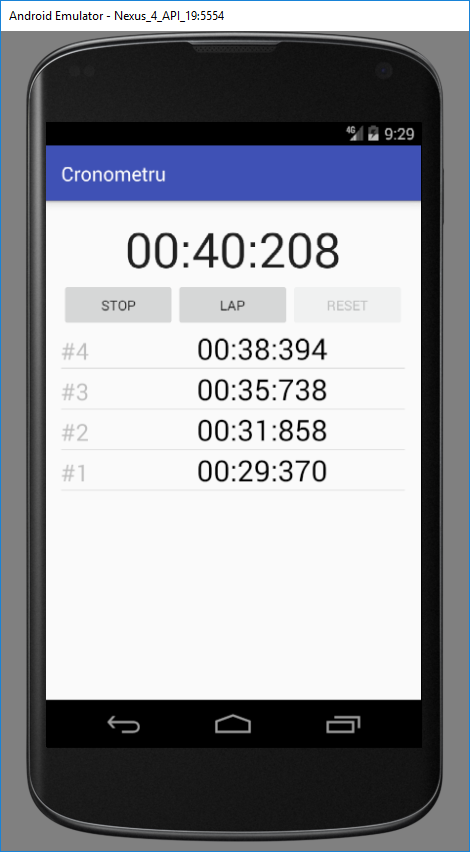
\includegraphics[scale=0.5]{imagini/3-laps}
	\centering
	\captionof{figure}{Înregistrările păstrate în listă}
\end{figure}

\begin{figure}[ht]
	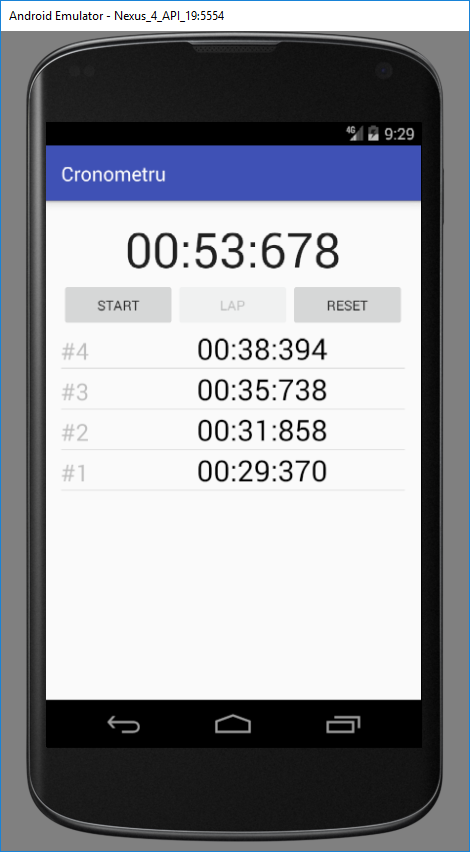
\includegraphics[scale=0.5]{imagini/4-stop}
	\centering
	\captionof{figure}{Cronometrul oprit}
\end{figure}

\begin{figure}[ht]
	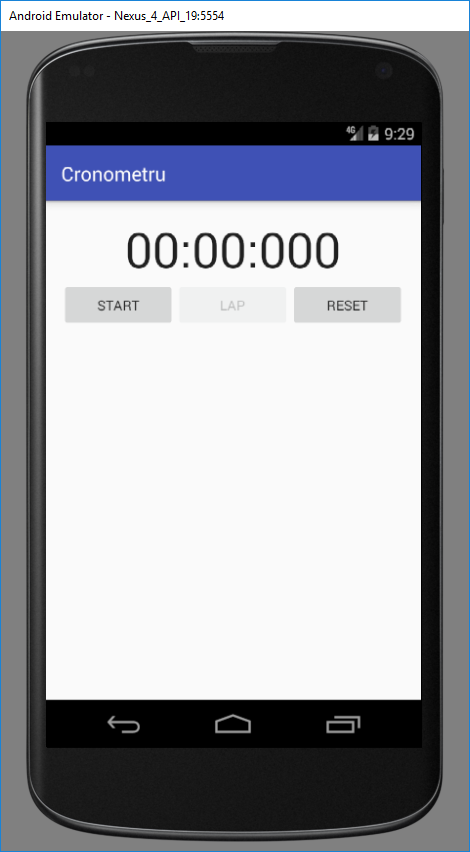
\includegraphics[scale=0.5]{imagini/5-reset}
	\centering
	\captionof{figure}{Cronometrul resetat}
\end{figure}

\clearpage